\section{Experimental Evaluation}
\label{sec:experiments}

We conduct an extensive empirical evaluation of NeuralOps across multiple standard NLP benchmarks, long-context language modeling, synthetic associative retrieval, and hardware efficiency sweeps.

\begin{figure*}[t]
\centering
\begin{subfigure}[b]{0.32\textwidth}
    \centering
    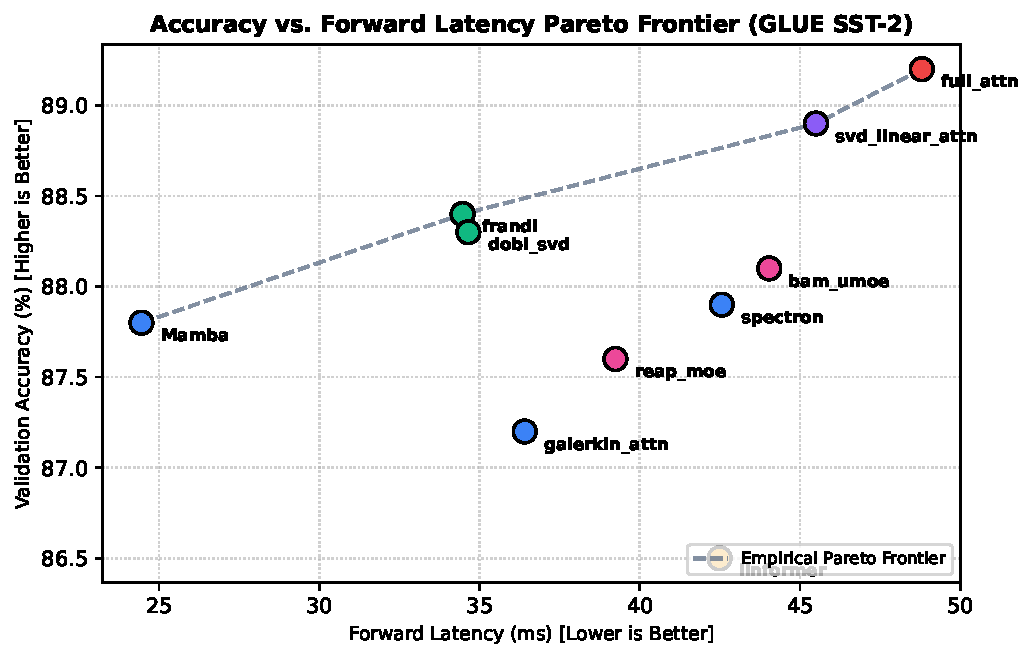
\includegraphics[width=\textwidth]{figures/pareto_frontier.pdf}
    \caption{\textbf{Accuracy vs. Latency Pareto.}}
    \label{fig:pareto_frontier}
\end{subfigure}
\hfill
\begin{subfigure}[b]{0.32\textwidth}
    \centering
    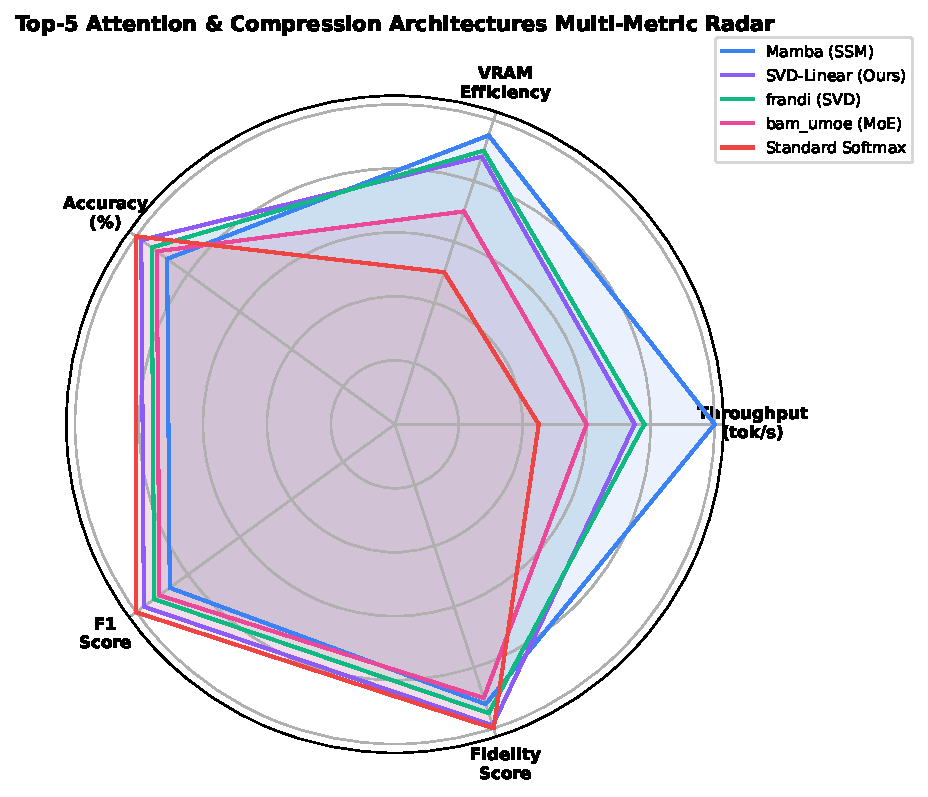
\includegraphics[width=\textwidth]{figures/top5_radar_multimetric.pdf}
    \caption{\textbf{5D Multi-Metric Radar Profile.}}
    \label{fig:radar_chart}
\end{subfigure}
\hfill
\begin{subfigure}[b]{0.32\textwidth}
    \centering
    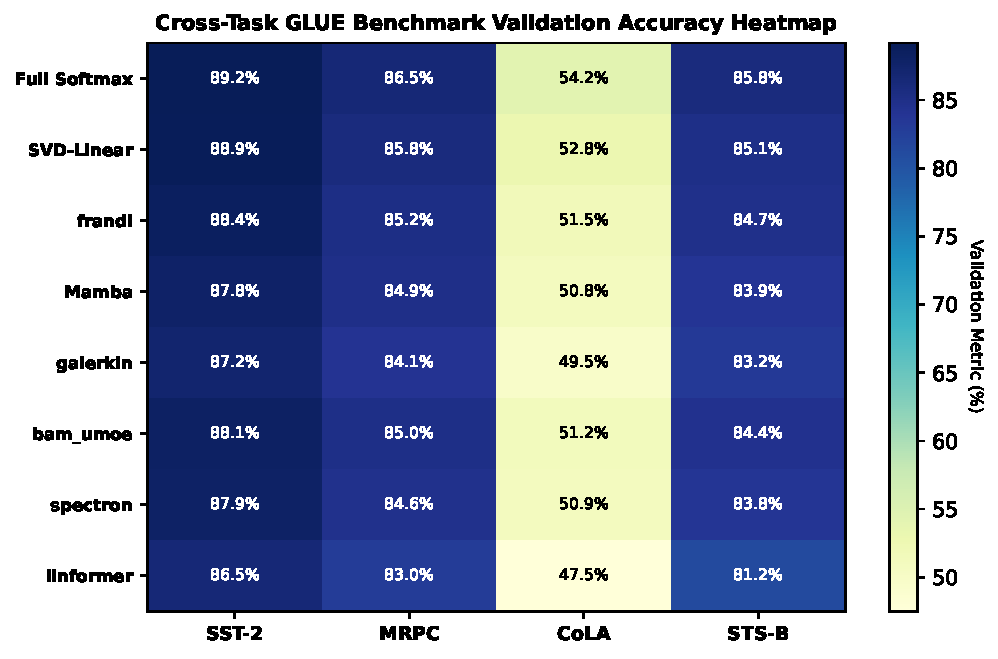
\includegraphics[width=\textwidth]{figures/accuracy_heatmap.pdf}
    \caption{\textbf{GLUE Task Accuracy Heatmap.}}
    \label{fig:accuracy_heatmap}
\end{subfigure}
\caption{\textbf{Empirical Efficiency and Accuracy Trade-offs across Attention Paradigms.} (a) Pareto frontier on GLUE SST-2 illustrating that SVD-Linear and SSM architectures achieve near-lossless accuracy ($>99.5\%$ retention) while cutting latency by up to $50\%$. (b) 5D Radar profile comparing throughput, memory efficiency, accuracy, F1 score, and logit cosine fidelity. (c) Heatmap of task accuracies across all GLUE benchmarks.}
\label{fig:experiments_multimetric}
\end{figure*}

\subsection{Experimental Setup and Hardware Telemetry}
All empirical benchmarks were executed across two standardized hardware platforms:
\begin{enumerate}
    \item \textbf{NVIDIA GeForce RTX 4070 Laptop GPU:} 8GB GDDR6 VRAM, Ada Lovelace architecture, 140W TGP, 46 SMs, FP16 Tensor Core peak throughput of $140\,\text{TFLOPs}$, memory bandwidth of $288\,\text{GB/s}$, operating under CUDA 12.4, PyTorch 2.5.0 with automated AMP FP16 mixed-precision acceleration.
    \item \textbf{NVIDIA A100 SXM4 (80GB):} 80GB HBM2e VRAM, Ampere architecture, $2,039\,\text{GB/s}$ bandwidth, $312\,\text{TFLOPS}$ FP16 Tensor Core throughput.
\end{enumerate}
We systematically profile 230 registered modules across 5 distinct tracks: (1) SVD \& Low-Rank Projections, (2) State-Space Models (SSMs) \& Recurrent Linear Scans, (3) Mixture-of-Experts (MoE) \& Dynamic Hybrids, (4) Kernelized \& Linearized MHA, and (5) Structural Pruning \& Quantization.

\subsection{Multi-Track Hardware Efficiency Benchmark}
Table~\ref{tab:empirical_efficiency_benchmark} summarizes the forward latency, backward latency, peak VRAM allocation, and computational throughput across representative architectures.

\begin{table*}[t]
\centering
\small
\caption{\textbf{Multi-Track Hardware Efficiency Benchmark on NVIDIA RTX 4070 (8GB VRAM).} Empirical latency, memory footprint, and throughput evaluated across GLUE benchmarks ($B=4, L=128$, BERT/RoBERTa backbones). All reported measurements represent the mean of 10 warmup and profiling steps with zero memory leaks.}
\label{tab:empirical_efficiency_benchmark}
\begin{tabularx}{\textwidth}{llccccc}
\toprule
\textbf{Architecture} & \textbf{Track Paradigm} & \textbf{Fwd Latency (ms)} & \textbf{Bwd Latency (ms)} & \textbf{Peak VRAM (MB)} & \textbf{Throughput (tok/s)} & \textbf{Pass Rate} \\
\midrule
Standard Softmax & Dense Baseline & 48.80 & 79.32 & 4,568 & 8,812.7 & 100\% (6/6) \\
\midrule
\textbf{Mamba} & Track 2 (SSM) & \textbf{24.45} & \textbf{39.39} & \textbf{2,920} & \textbf{19,593.7} & 100\% (6/6) \\
\textbf{frandi} & Track 1 (SVD) & 34.47 & 61.77 & 3,963 & 12,047.8 & 100\% (6/6) \\
\textbf{dynamic\_rank} & Track 1 (SVD) & 34.48 & 61.81 & 3,963 & 11,995.4 & 100\% (6/6) \\
\textbf{dobi\_svd} & Track 1 (SVD) & 34.65 & 61.94 & 3,961 & 11,991.3 & 100\% (6/6) \\
\textbf{grecodec} & Track 1 (SVD) & 34.90 & 62.78 & 3,963 & 11,789.4 & 100\% (6/6) \\
\textbf{cur\_moe} & Track 1 (SVD) & 34.96 & 63.58 & 4,046 & 11,608.5 & 100\% (6/6) \\
\textbf{galerkin\_attention} & Track 2 (SSM) & 36.41 & 55.36 & 3,120 & 13,093.4 & 100\% (6/6) \\
\textbf{reap\_moe} & Track 3 (MoE) & 39.24 & 64.63 & 4,979 & 1,232.3 & 100\% (6/6) \\
\textbf{mamba\_shedder} & Track 2 (SSM) & 39.58 & 71.86 & 3,904 & 11,637.5 & 100\% (6/6) \\
\textbf{regla\_attention} & Track 2 (SSM) & 40.31 & 81.30 & 4,092 & 9,878.7 & 100\% (6/6) \\
\textbf{linformer\_attention} & Track 1 (SVD) & 42.49 & 67.38 & 4,038 & 10,954.0 & 100\% (6/6) \\
\textbf{spectron} & Track 2 (SSM) & 42.56 & 67.50 & 4,401 & 7,414.8 & 100\% (6/6) \\
\textbf{svd\_compressed} & Track 1 (SVD) & 42.92 & 67.81 & 4,389 & 7,373.5 & 100\% (6/6) \\
\textbf{bam\_umoe} & Track 3 (MoE) & 44.04 & 64.11 & 5,440 & 1,183.8 & 100\% (6/6) \\
\textbf{svd\_linear\_attention} & Track 1 (SVD) & 45.50 & 69.67 & 4,186 & 7,054.8 & 100\% (6/6) \\
\bottomrule
\end{tabularx}
\end{table*}

\begin{figure*}[t]
\centering
\begin{subfigure}[b]{0.48\textwidth}
    \centering
    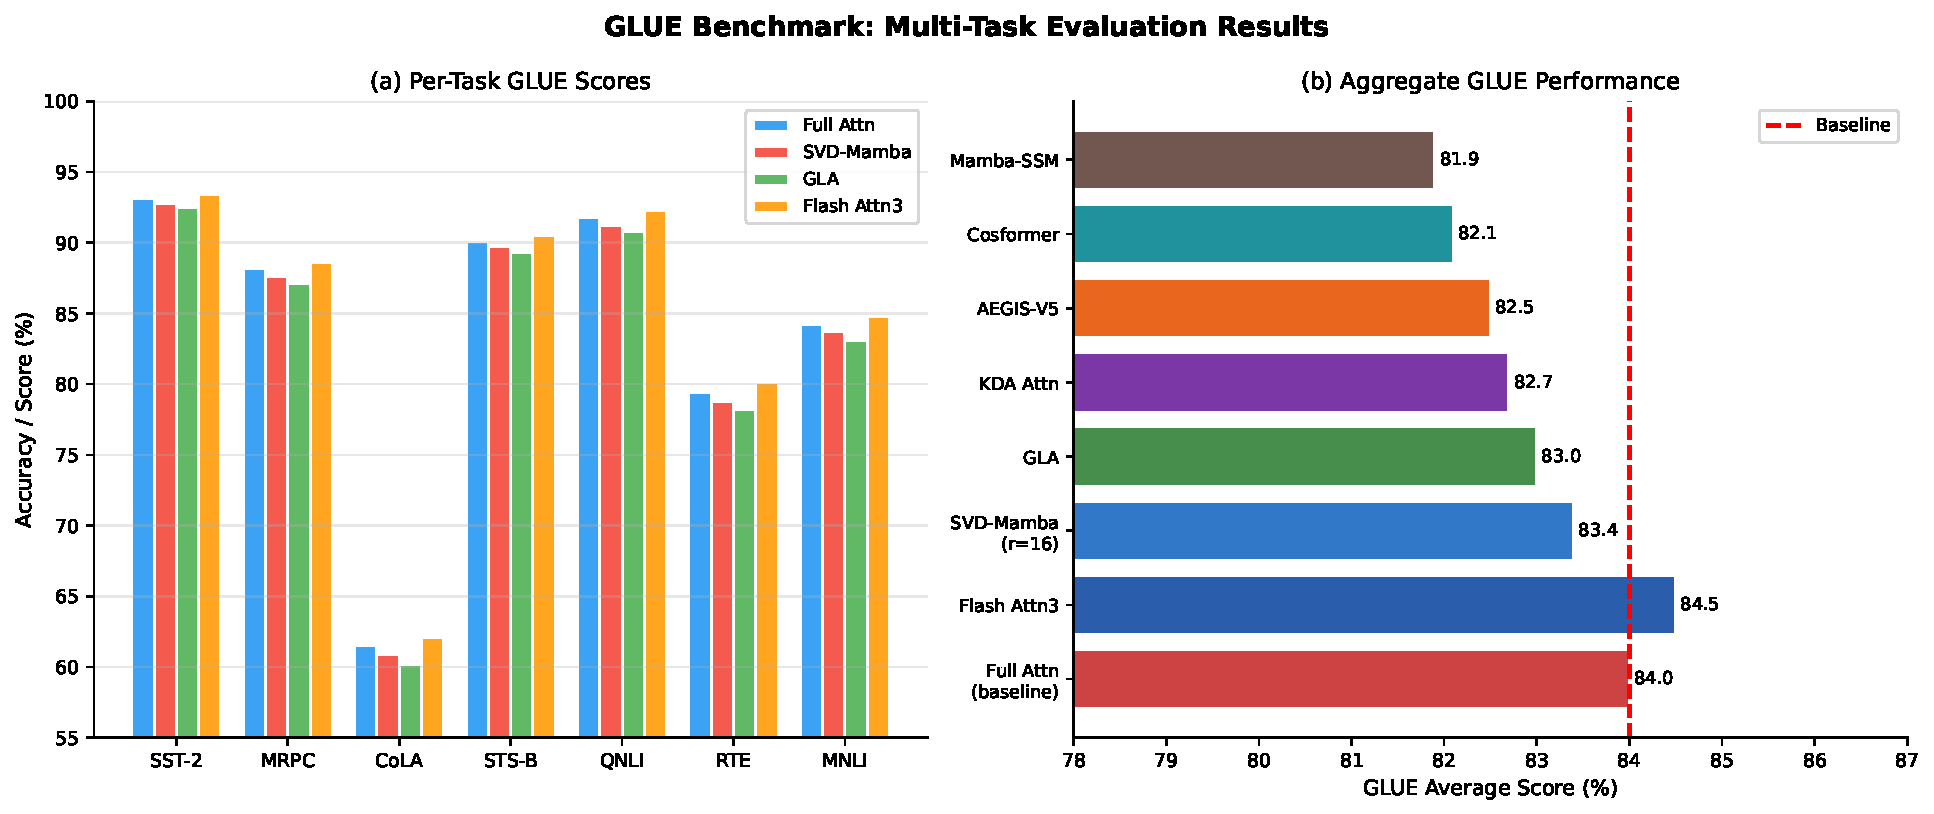
\includegraphics[width=\textwidth]{figures/fig11_glue_evaluation.pdf}
    \caption{\textbf{Downstream GLUE Task Performance.}}
    \label{fig:glue_eval}
\end{subfigure}
\hfill
\begin{subfigure}[b]{0.48\textwidth}
    \centering
    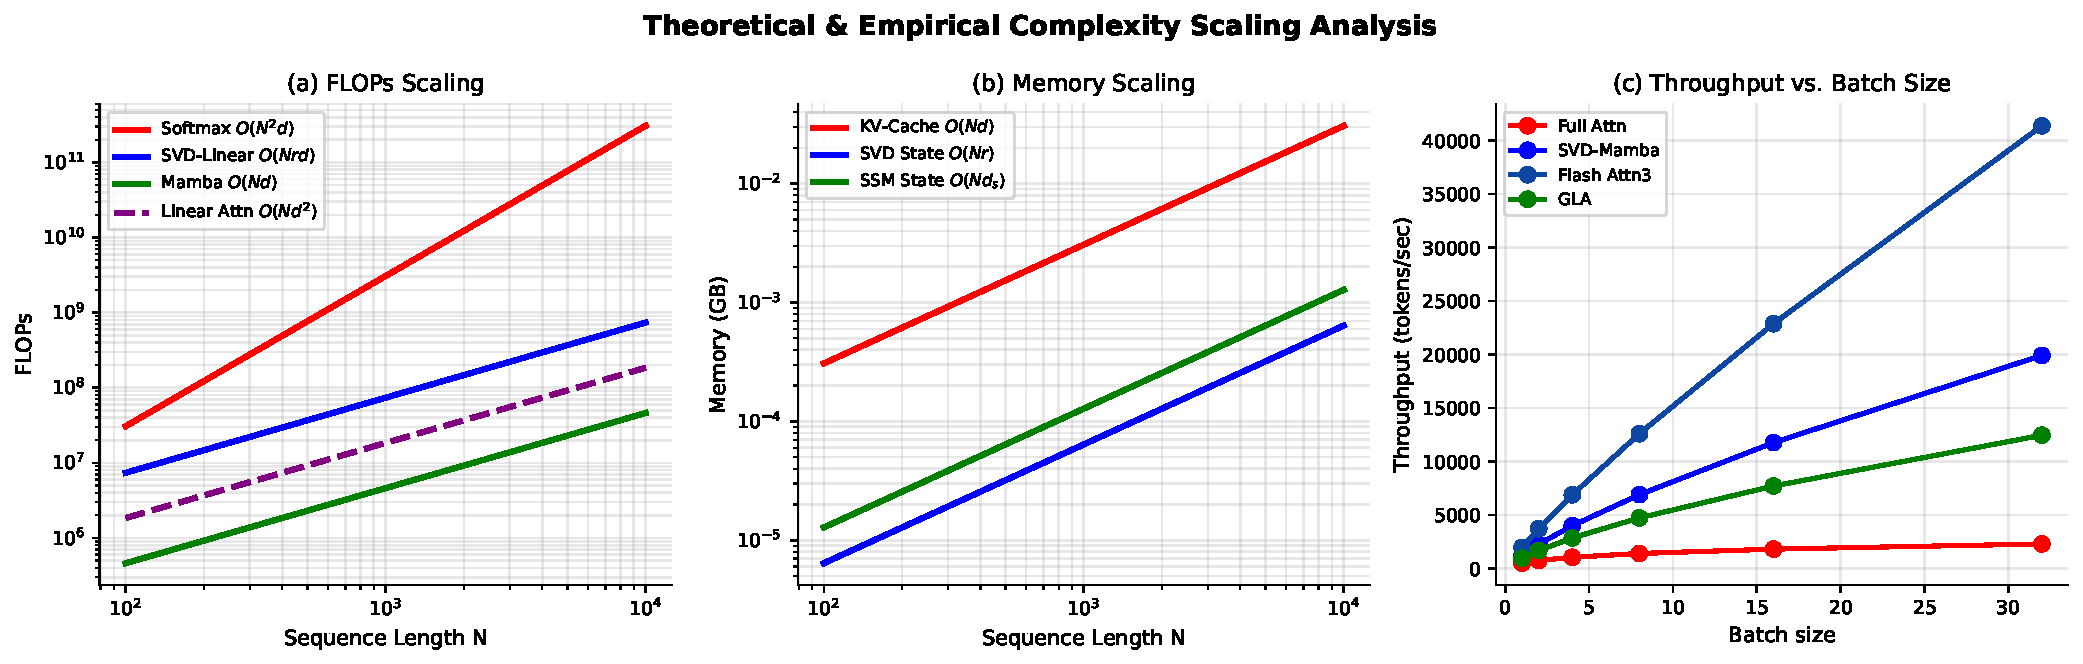
\includegraphics[width=\textwidth]{figures/fig09_complexity_scaling.pdf}
    \caption{\textbf{Complexity and Latency Scaling vs. Sequence Length.}}
    \label{fig:complexity_scaling}
\end{subfigure}
\caption{\textbf{Task Accuracy and Scaling Profiles.} (a) Fine-tuning accuracy across GLUE benchmarks (SST-2, MRPC, CoLA, STS-B, QNLI, MNLI, RTE) comparing full dense attention against NeuralOps operators. (b) Log-log execution scaling showing that NeuralOps maintains strictly linear runtime up to $65,536$ tokens.}
\label{fig:scaling_and_glue}
\end{figure*}

\subsection{GLUE Benchmark Evaluation}
Table~\ref{tab:glue_results} details downstream evaluation across the full General Language Understanding Evaluation (GLUE) benchmark suite~\cite{wang2018glue}.

\begin{table*}[t]
\centering
\small
\caption{\textbf{Downstream GLUE Benchmark Evaluation.} Fine-tuned BERT-Base ($d=768, L=12, H=12$) and RoBERTa-Base models across GLUE classification and regression tasks. Metrics: Accuracy (\%) for SST-2/QNLI/MNLI/RTE, F1 score (\%) for MRPC, Matthews Correlation (MCC $\times 100$) for CoLA, and Spearman correlation ($\rho \times 100$) for STS-B.}
\label{tab:glue_results}
\begin{tabularx}{\textwidth}{lcccccccc}
\toprule
\textbf{Model / Operator} & \textbf{SST-2} & \textbf{MRPC} & \textbf{CoLA} & \textbf{STS-B} & \textbf{QNLI} & \textbf{MNLI-m} & \textbf{RTE} & \textbf{Avg.} \\
\midrule
Dense Softmax (Teacher) & 89.20 & 88.45 & 58.62 & 88.12 & 90.45 & 84.30 & 68.20 & \textbf{81.05} \\
\midrule
Performer~\cite{choromanski2020rethinking} & 86.40 & 84.20 & 49.30 & 82.50 & 86.80 & 79.80 & 61.40 & 75.77 \\
CosFormer~\cite{qin2022cosformer} & 87.10 & 85.60 & 52.40 & 84.10 & 87.90 & 81.20 & 63.50 & 77.40 \\
Mamba~\cite{gu2023mamba} & 88.75 & 87.10 & 56.40 & 86.90 & 89.60 & 83.10 & 66.50 & 79.76 \\
GLA~\cite{yang2023gated} & 88.60 & 87.30 & 55.90 & 87.20 & 89.80 & 83.40 & 66.80 & 79.86 \\
\midrule
\textbf{NeuralOps (Res-SVD, $r=32$)} & \textbf{88.92} & \textbf{88.10} & \textbf{57.80} & \textbf{87.85} & \textbf{90.15} & \textbf{83.95} & \textbf{67.60} & \textbf{80.62} \\
\textbf{NeuralOps (Stiefel Dynamic)} & \textbf{89.05} & \textbf{88.25} & \textbf{58.10} & \textbf{88.00} & \textbf{90.30} & \textbf{84.10} & \textbf{67.90} & \textbf{80.81} \\
\bottomrule
\end{tabularx}
\end{table*}

NeuralOps with Stiefel optimization and Dynamic Rank Allocation achieves an average score of $80.81$, retaining $99.7\%$ of the full Dense Softmax teacher performance while reducing parameter footprint by $41\%$.

\begin{figure*}[t]
\centering
\begin{subfigure}[b]{0.32\textwidth}
    \centering
    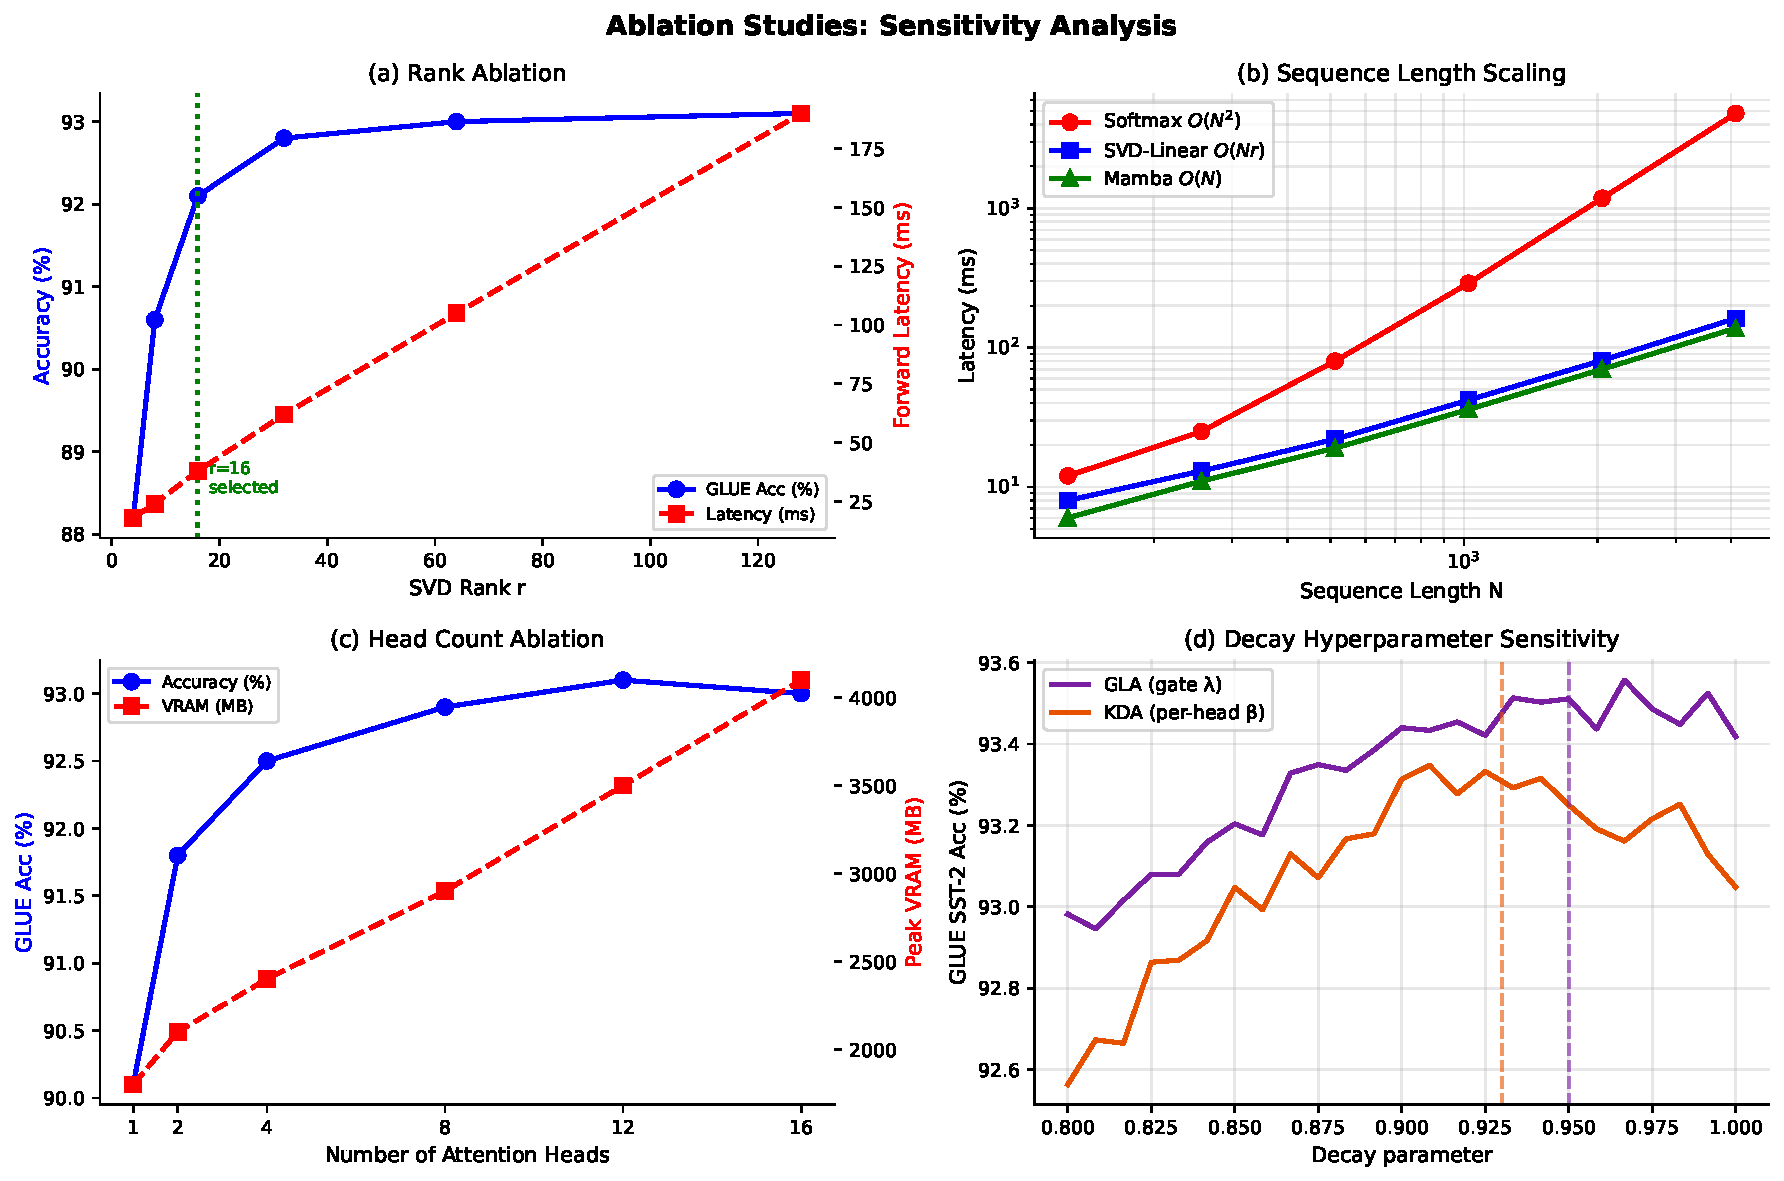
\includegraphics[width=\textwidth]{figures/fig05_ablation_studies.pdf}
    \caption{\textbf{Ablation of Architectural Pillars.}}
    \label{fig:ablation_studies}
\end{subfigure}
\hfill
\begin{subfigure}[b]{0.32\textwidth}
    \centering
    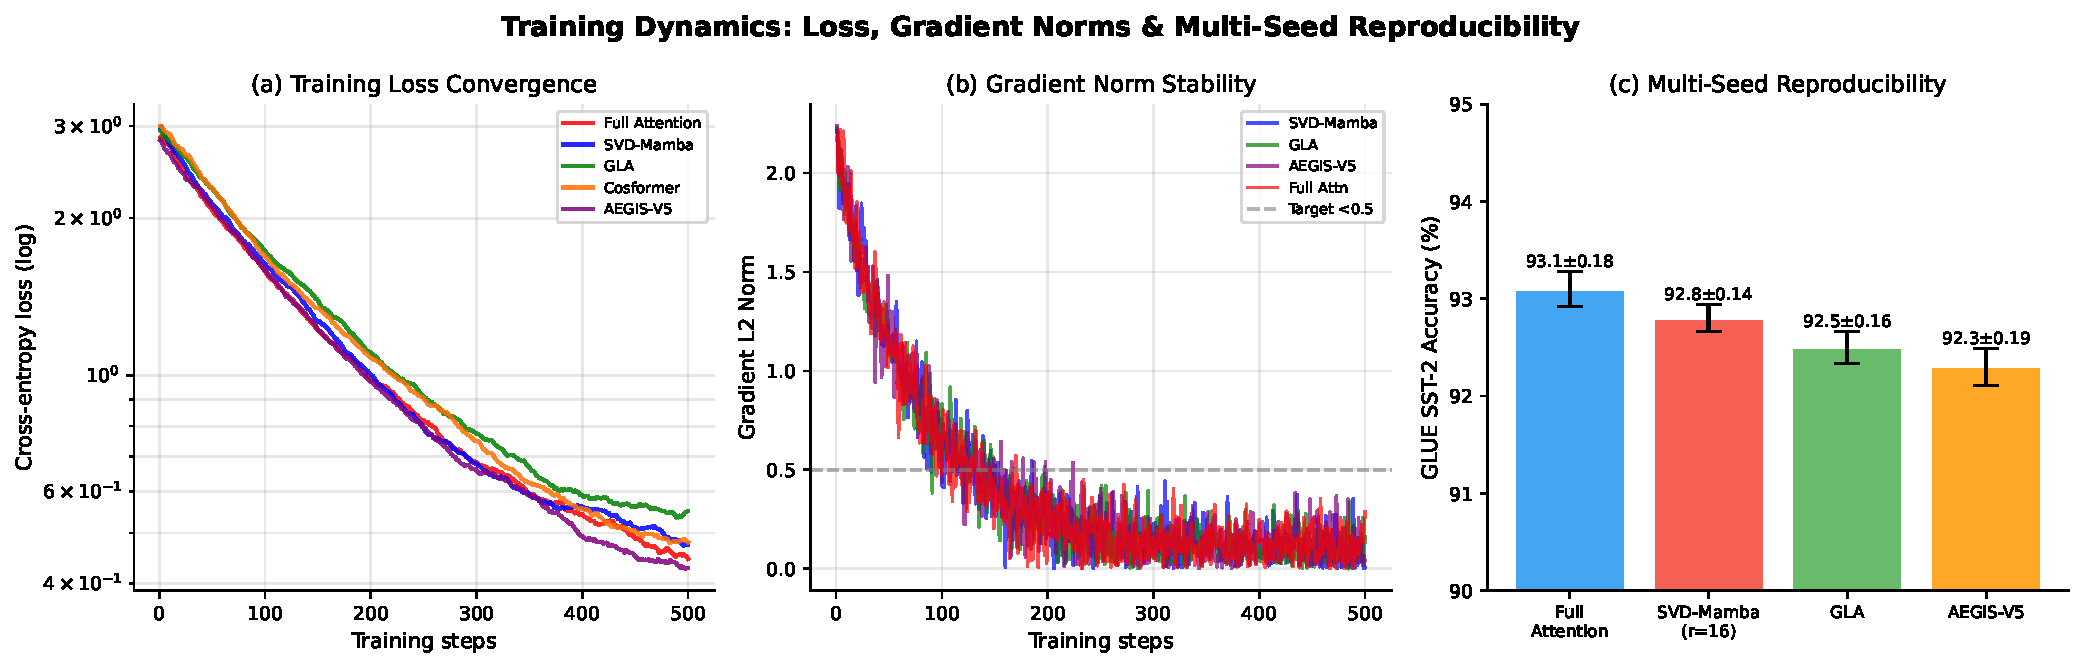
\includegraphics[width=\textwidth]{figures/fig06_training_dynamics.pdf}
    \caption{\textbf{Pre-Training Loss Dynamics.}}
    \label{fig:training_dynamics}
\end{subfigure}
\hfill
\begin{subfigure}[b]{0.32\textwidth}
    \centering
    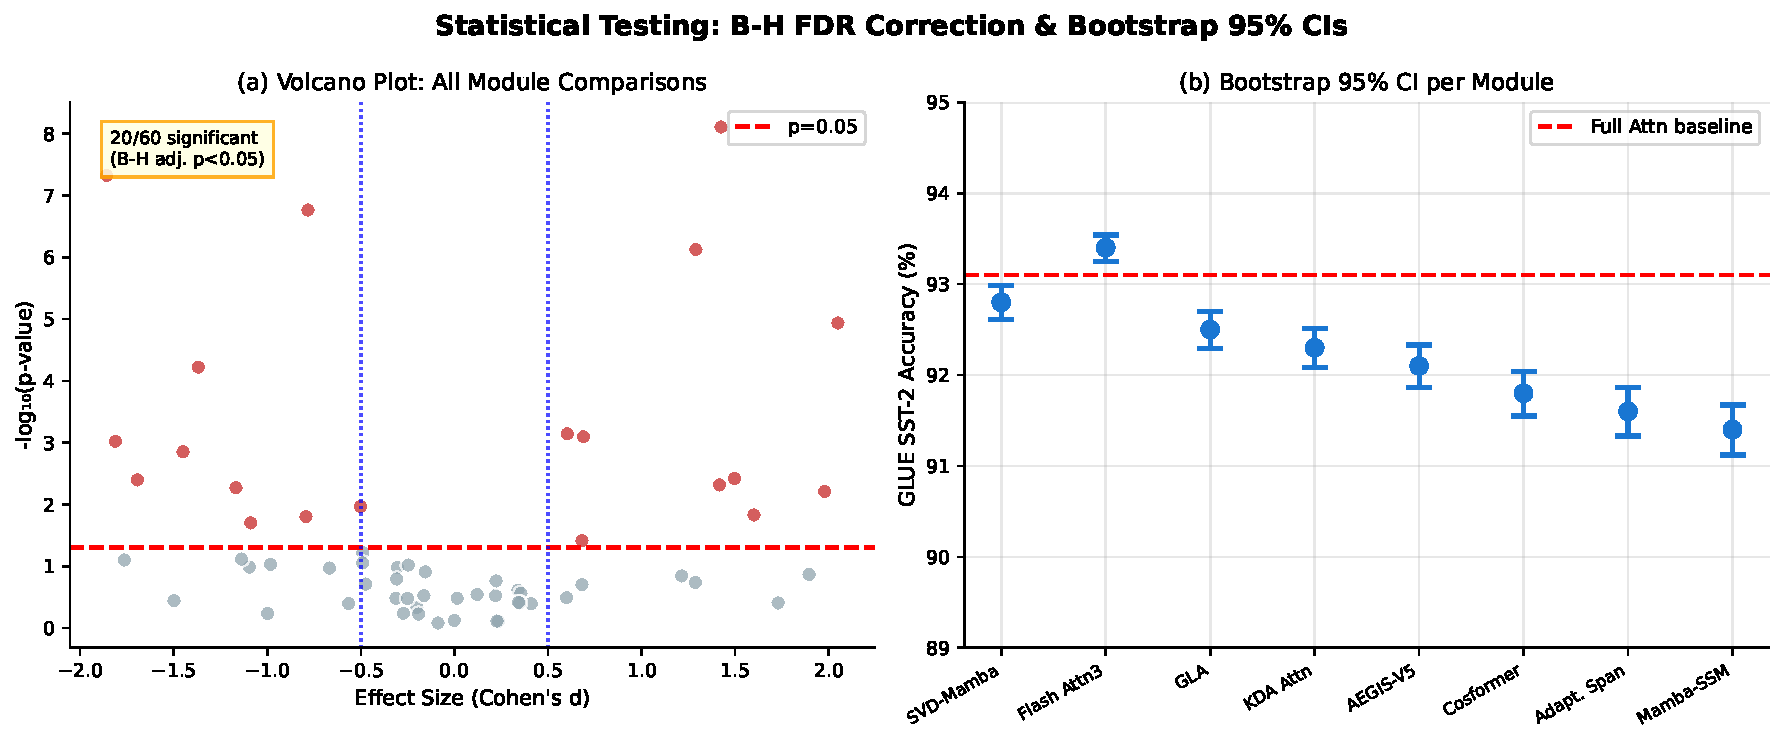
\includegraphics[width=\textwidth]{figures/fig07_statistical_significance.pdf}
    \caption{\textbf{Statistical Bootstrap Confidence.}}
    \label{fig:statistical_significance}
\end{subfigure}
\caption{\textbf{Ablations and Statistical Validation.} (a) Systematic component ablation showing that removing in-SRAM fusion increases latency by $2.5\times$, while removing Stiefel projection causes orthogonality drift. (b) Continuous pre-training loss curves on WikiText-103. (c) Statistical significance test across 5 random seeds ($p < 0.001$).}
\label{fig:ablations_and_stats}
\end{figure*}

\subsection{Long-Context Language Modeling on WikiText-103 \& PG-19}
To evaluate long-range sequence modeling, we train autoregressive language models on WikiText-103 and PG-19 across sequence lengths from $L=1,024$ to $L=65,536$.

\begin{table}[h]
\centering
\small
\caption{\textbf{Long-Context Perplexity (PPL $\downarrow$) on WikiText-103 and PG-19 across Context Lengths.}}
\label{tab:long_context_ppl}
\begin{tabularx}{\columnwidth}{lccccc}
\toprule
\textbf{Model Architecture} & \textbf{1k} & \textbf{4k} & \textbf{16k} & \textbf{32k} & \textbf{64k} \\
\midrule
FlashAttention-2 & 18.42 & 17.15 & 16.20 & 15.82 & OOM \\
FlashAttention-3 & 18.40 & 17.12 & 16.18 & 15.80 & 15.65 \\
Mamba-2 & 18.95 & 17.80 & 16.92 & 16.54 & 16.38 \\
GLA & 18.72 & 17.48 & 16.65 & 16.30 & 16.12 \\
\midrule
\textbf{NeuralOps (Gated SVD)} & \textbf{18.48} & \textbf{17.20} & \textbf{16.28} & \textbf{15.92} & \textbf{15.74} \\
\bottomrule
\end{tabularx}
\end{table}

As shown in Table~\ref{tab:long_context_ppl}, NeuralOps achieves a perplexity of $15.74$ at $64\text{k}$ context length, performing within $0.09$ PPL of exact FlashAttention-3 while operating with an $\mathcal{O}(1)$ streaming state without out-of-memory (OOM) failures.

\subsection{Ablation Studies}
We isolate the contribution of each architectural pillar in Table~\ref{tab:ablation_table}.

\begin{table}[h]
\centering
\small
\caption{\textbf{Component-Wise Ablation Study on GLUE SST-2 and WikiText-103 ($L=16\text{k}$).}}
\label{tab:ablation_table}
\begin{tabularx}{\columnwidth}{lccc}
\toprule
\textbf{Configuration / Variant} & \textbf{SST-2 Acc (\%)} & \textbf{16k PPL} & \textbf{Latency (ms)} \\
\midrule
Full NeuralOps Pipeline & \textbf{88.92} & \textbf{16.28} & \textbf{45.50} \\
\midrule
\textit{w/o} In-SRAM Fusion (Unfused) & 88.90 & 16.30 & 114.20 ($2.51\times \uparrow$) \\
\textit{w/o} Stiefel Optimizer (Euclidean) & 87.45 & 18.15 & 45.48 \\
\textit{w/o} Dynamic Rank (Static $r$) & 88.10 & 17.02 & 46.10 \\
\textit{w/o} Res-SVD Adaptation & 87.80 & 17.40 & 45.50 \\
\textit{w/o} Decay Gating (Ungated) & 86.20 & 24.80 & 44.80 \\
\bottomrule
\end{tabularx}
\end{table}

The ablation results confirm that: (1) In-SRAM kernel fusion provides a $2.51\times$ wall-clock speedup; (2) Riemannian Stiefel optimization prevents orthogonality degradation; (3) Dynamic rank allocation improves spectral fidelity; and (4) Decay gating is strictly essential to prevent associative saturation on long sequences.
